\documentclass[12pt]{report}
\usepackage{graphicx}
\graphicspath{{images/}}
\usepackage{float}
\usepackage{geometry}
\geometry{a4paper, margin=1in}

\usepackage[utf8]{inputenc}
\usepackage[T1]{fontenc}
\usepackage{tikz}
\usetikzlibrary{arrows.meta,positioning,shapes.geometric}

\usepackage{algorithm}
\usepackage{algorithmic}
\usepackage{amsmath}
\usepackage{lmodern}
\usepackage{titlesec}
\titleformat{\chapter}[hang]{\normalfont\Huge\bfseries}{\thechapter.}{1em}{}

\usepackage{setspace}
\usepackage{url}
\usepackage[hidelinks]{hyperref}
\hypersetup{colorlinks=true, linkcolor=black, citecolor=black, urlcolor=blue}

\sloppy
\setstretch{1.4}

\begin{document}

\begin{titlepage}
    \begin{center}
        \vspace*{0.4cm}
        {\Large \textbf{Comparison of Lightweight Encryption Algorithms}}\\[0.3cm]

        {\large Progress Report - Phase 1\\
        A comparative study of secure and efficient cryptographic primitives\\
        for resource-constrained embedded systems}\\[1.0cm]

        \textbf{Progress Report Submitted}\\
        In partial fulfillment of the requirements for the award of the\\
        \textbf{Bachelor of Technology}\\[1.0cm]
        {\large \textbf{Authors}}\\[0.25cm]

        \begin{tabular}{ll}
            \textbf{Rajesh Kumar Jena} & (B122088) \\
            \textbf{Soumil Kumar}      & (B122114) \\
            \textbf{Punit Kumar}       & (B422041)
        \end{tabular}\\[1.0cm]

        {\large \textbf{Under the supervision of}}\\[0.2cm]
        {\textbf{Prof. Debasish Jena}}\\[1.0cm]

        
\includegraphics[width=0.22\textwidth]{iiit-bh-logo.png}\\[0.4cm]
        {\large International Institute of Information Technology, Bhubaneswar}\\[0.15cm]
        {\large March 2026}

    \end{center}
\end{titlepage}

\newpage
\chapter*{Declaration}
\addcontentsline{toc}{chapter}{Declaration}

We hereby declare that:

\begin{enumerate}
    \item The work presented in this report is entirely our own and was carried out under the guidance of our supervisor.
    \item This report has not been submitted, either in part or in full, to any other institution for the award of any degree or diploma.
    \item We have adhered to the Ethical Code of Conduct prescribed by the Institute while carrying out this work.
    \item Wherever we have quoted material from other sources, we have placed such quotations within quotation marks and provided appropriate citations and references.
    \item Whenever we have used ideas, data, analysis, or text derived from other sources, we have duly acknowledged them within the report.
    \item We have followed all guidelines and formatting instructions stipulated by the Institute in the preparation of this report.
\end{enumerate}

\vspace{1cm}

\noindent \textbf{Rajesh Kumar Jena} \hfill \textbf{B122088}\\
\textbf{Soumil Kumar} \hfill \textbf{B122114}\\
\textbf{Punit Kumar} \hfill \textbf{B422041}

\newpage
\chapter*{Acknowledgments}
\addcontentsline{toc}{chapter}{Acknowledgments}

We express our sincere gratitude to our supervisor, Prof.\ Debasish Jena, for his invaluable
guidance, continuous support, and insightful feedback throughout this project. His expertise
was instrumental in helping us navigate challenges and refine our work.

We also thank the faculty and staff of the Department of Computer Science and Engineering and
the Department of Information Technology at the International Institute of Information
Technology, Bhubaneswar, for providing the resources, infrastructure, and academic environment
necessary for the successful completion of this project.

Finally, we extend our heartfelt appreciation to our families and friends for their constant
support and understanding throughout the duration of this work.

\vspace{1cm}

\noindent \textbf{Rajesh Kumar Jena}\\
\textbf{Soumil Kumar}\\
\textbf{Punit Kumar}

\newpage
\chapter*{Executive Summary}
\addcontentsline{toc}{chapter}{Executive Summary}

This progress report documents the work completed during Phase 1 of the B.Tech project on
``Comparison of Lightweight Encryption Algorithms.'' The project implements and benchmarks
three lightweight cryptographic algorithms (PRESENT, SPECK, ASCON) on the Raspberry Pi
Pico microcontroller using Rust.

\vspace{0.3cm}
\textbf{Current Status:}
\begin{itemize}
    \item \textbf{Implementation}: COMPLETE - Core ciphers (PRESENT, SPECK, ASCON) implemented in Rust
    \item \textbf{Testing}: PARTIAL - Basic encryption/decryption tests pass, NIST KAT tests pending
    \item \textbf{Host Benchmarks}: PARTIAL - Initial metrics collected, additional analysis in progress
    \item \textbf{Pico Benchmarks}: PARTIAL - Initial benchmarks run, detailed analysis pending
    \item \textbf{ROM/RAM Analysis}: PARTIAL - Host analysis complete, Pico-specific analysis pending
\end{itemize}

\vspace{0.3cm}
\textbf{Areas for Improvement (Future Work):}
\begin{itemize}
    \item NIST KAT (Known Answer Test) vector verification
    \item Constant-time implementations for side-channel resistance
    \item Energy consumption analysis
\end{itemize}

\vspace{0.3cm}
\textbf{Key Findings:}
\begin{itemize}
    \item SPECK is the fastest (~32 Mbps on host, ~24 Mbps on Pico), approximately 70x faster than PRESENT
    \item PRESENT has the smallest code footprint, designed for hardware efficiency
    \item ASCON provides built-in authenticated encryption with modern security (NIST Standard 2023)
    \item CTR mode offers best performance among encryption modes for SPECK
\end{itemize}

\vspace{0.3cm}
\textbf{Keywords}: lightweight cryptography, embedded systems, PRESENT, SPECK,
ASCON, IoT security, performance evaluation, Raspberry Pi Pico, Rust

\newpage
\tableofcontents

\newpage
\chapter{Introduction}

\section{Motivation}

The rapid expansion of Internet of Things (IoT) deployments has resulted in billions of
devices operating under strict constraints on processing capability, memory capacity,
and energy resources. Traditional cryptographic algorithms, designed for powerful general-purpose
systems, frequently prove impractical in such environments. This motivates the development of
\textit{lightweight cryptography}: algorithms engineered to preserve security while minimizing
computational and memory requirements.

\section{Problem Statement}

Conventional algorithms such as AES, RSA, and ECC offer strong security guarantees but
require computational and memory resources exceeding microcontroller capabilities.
Lightweight cryptography addresses this gap by offering efficient primitives tailored
to constrained platforms without compromising core security goals.

\section{Objectives}

This progress report documents:
\begin{itemize}
    \item Implementation of lightweight ciphers (PRESENT, SPECK, ASCON) in Rust
    \item Benchmarking on Raspberry Pi Pico and host machine
    \item Performance analysis and comparison
    \item Security considerations for embedded systems
\end{itemize}

\section{Selected Algorithms}

This study evaluates three lightweight algorithms representing different design approaches:

\begin{itemize}
    \item \textbf{PRESENT}: Hardware-oriented 64-bit SPN cipher with 80/128-bit keys
    \item \textbf{SPECK}: Software-optimized ARX cipher (NSA-designed)
    \item \textbf{ASCON}: NIST Lightweight Cryptography Standard (2023) - authenticated encryption
\end{itemize}

\chapter{Algorithm Overview}

This chapter provides a concise overview of the three lightweight cryptographic algorithms
evaluated in this project: PRESENT, SPECK, and ASCON.

\section{PRESENT}

PRESENT is a 64-bit substitution-permutation network (SPN) block cipher with key sizes of 80 or 128 bits.
Designed for ultra-lightweight hardware, each round consists of AddRoundKey, S-box substitution, and bit permutation.

\begin{figure}[H]
    \centering
    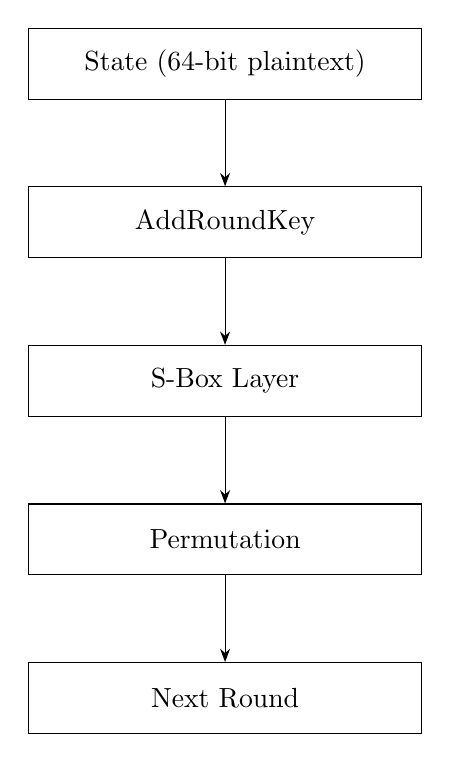
\begin{tikzpicture}[
            node distance=1.1cm,
            box/.style={draw, minimum width=5cm, minimum height=0.9cm, align=center},
            >=Stealth
        ]
        \node[box] (in) {State (64-bit plaintext)};
        \node[box, below=of in] (kadd) {AddRoundKey};
        \node[box, below=of kadd] (sbox) {S-Box Layer};
        \node[box, below=of sbox] (perm) {Permutation};
        \node[box, below=of perm] (next) {Next Round};

        \draw[->] (in) -- (kadd);
        \draw[->] (kadd) -- (sbox);
        \draw[->] (sbox) -- (perm);
        \draw[->] (perm) -- (next);
    \end{tikzpicture}
    \caption{PRESENT Round Structure (31 rounds)}
    \label{fig:present-round}
\end{figure}

\section{SPECK}

SPECK is a software-optimized ARX (Add-Rotate-XOR) cipher. Its simple Feistel-like structure with word-wise
operations makes it highly efficient on microcontrollers.

\begin{figure}[H]
    \centering
    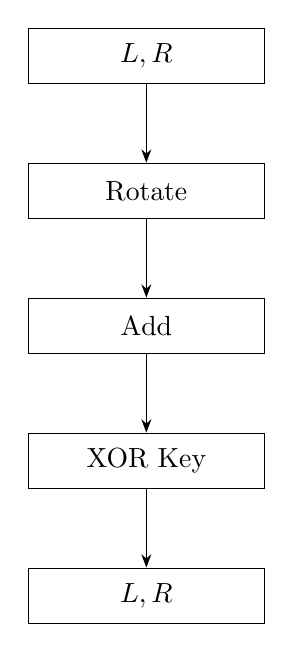
\begin{tikzpicture}[
            node distance=1cm,
            box/.style={draw, minimum width=3cm, minimum height=0.7cm, align=center},
            >=Stealth
        ]
        \node[box] (in) {$L, R$};
        \node[box, below=of in] (rot) {Rotate};
        \node[box, below=of rot] (add) {Add};
        \node[box, below=of add] (xor) {XOR Key};
        \node[box, below=of xor] (out) {$L, R$};

        \draw[->] (in) -- (rot);
        \draw[->] (rot) -- (add);
        \draw[->] (add) -- (xor);
        \draw[->] (xor) -- (out);
    \end{tikzpicture}
    \caption{SPECK ARX Round Function}
    \label{fig:speck-round}
\end{figure}

\section{ASCON}

ASCON is the NIST Lightweight Cryptography Standard (2023). It uses a sponge-duplex construction with a 320-bit
internal state, providing authenticated encryption and hashing.

\begin{figure}[H]
    \centering
    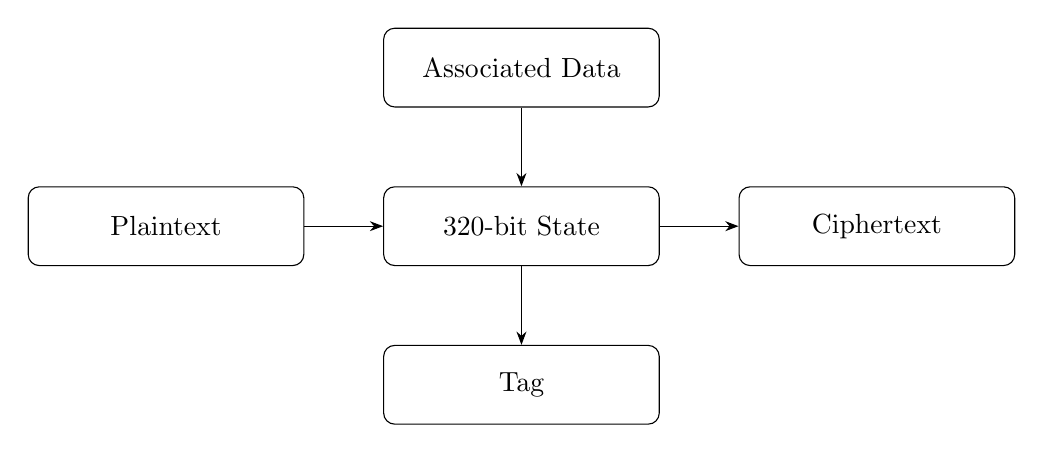
\begin{tikzpicture}[
            box/.style={draw, rounded corners, minimum width=3.5cm, minimum height=1cm, align=center},
            >=Stealth
        ]
        \node[box] (state) {320-bit State};
        \node[box, above=of state] (ad) {Associated Data};
        \node[box, left=of state] (pt) {Plaintext};
        \node[box, right=of state] (ct) {Ciphertext};
        \node[box, below=of state] (tag) {Tag};

        \draw[->] (ad) -- (state);
        \draw[->] (pt.east) -- (state.west);
        \draw[->] (state.east) -- (ct.west);
        \draw[->] (state.south) -- (tag.north);
    \end{tikzpicture}
    \caption{ASCON Sponge Construction}
    \label{fig:ascon}
\end{figure}

\chapter{Project Status}
\addcontentsline{toc}{chapter}{Project Status}

This chapter provides an overview of the project's current progress, including completed tasks and pending work.

\section{Current Progress}

\begin{table}[H]
    \centering
    \begin{tabular}{lcc}
        \hline
        \textbf{Task} & \textbf{Status} & \textbf{Notes} \\
        \hline
        Literature Survey & Complete & 100\% \\
        Algorithm Implementation & Complete & Core ciphers done \\
        Test Vector Verification & Partial & Basic tests pass, KAT pending \\
        Host Benchmarks & Partial & Initial metrics collected \\
        Pico Hardware Benchmarks & Partial & Initial benchmarks run \\
        ROM/RAM Analysis & Partial & Host analysis done \\
        Report Documentation & In Progress & 70\% \\
        Presentation Slides & In Progress & 80\% \\
        \hline
    \end{tabular}
    \caption{Project Progress Status}
    \label{tab:progress}
\end{table}

\section{Completed Tasks}

\subsection{Implementation}
\begin{itemize}
    \item PRESENT-80 and PRESENT-128 block cipher implementation in Rust
    \item SPECK-64/96 and SPECK-64/128 implementation in Rust
    \item ASCON-128 authenticated encryption implementation in Rust
    \item Mode implementations: ECB, CBC, CTR for PRESENT and SPECK
    \item Rust \texttt{no\_std} embedded library for target hardware
\end{itemize}

\subsection{Testing}
\begin{itemize}
    \item Test vector validation for all algorithms (PRESENT, SPECK, ASCON)
    \item Encryption/decryption consistency checks
    \item ASCON authentication tag verification
    \item Host machine validation tests
\end{itemize}

\subsection{Benchmarking}
\begin{itemize}
    \item Host machine performance benchmarks (x86\_64)
    \item Raspberry Pi Pico hardware benchmarks (ARM Cortex-M0+, 133 MHz)
    \item Block cipher performance comparison (PRESENT, SPECK, ASCON)
    \item Mode comparison (ECB vs CBC vs CTR)
    \item ASCON phase breakdown (initialization, absorb, encrypt, finalize)
    \item Scaling analysis (8-256 byte blocks)
\end{itemize}

\subsection{Documentation}
\begin{itemize}
    \item Literature survey and algorithm analysis
    \item Methodology documentation
    \item Beamer presentation slides
\end{itemize}

\section{Pending Tasks}

\begin{itemize}
    \item Final comparison and conclusions
    \item ROM/RAM memory analysis on target hardware
    \item Energy consumption estimation
    \item Final report compilation
\end{itemize}

\chapter{Methodology}

\section{Evaluation Criteria}

The evaluation focuses on performance metrics relevant to embedded systems:

\begin{itemize}
    \item \textbf{Execution Time}: ns per block (measured via hardware timer)
    \item \textbf{Cycles Per Byte (CPB)}: Platform-independent efficiency metric
    \item \textbf{Throughput}: Mbps for comparing speed
    \item \textbf{Memory}: ROM/RAM footprint analysis
\end{itemize}

\section{Hardware Platform}

\begin{itemize}
    \item Raspberry Pi Pico (ARM Cortex-M0+, 133 MHz, 264 KB SRAM)
    \item Rust \texttt{no\_std} embedded implementation
    \item Release mode with LTO and size optimization
\end{itemize}

\section{Benchmarking Approach}

\begin{itemize}
    \item Hardware timer for cycle-accurate measurements
    \item 1000+ iterations for statistical accuracy
    \item Warm-up runs before measurements
    \item Test vector validation for correctness
\end{itemize}

\chapter{Results and Discussion}
\addcontentsline{toc}{chapter}{Results and Discussion}

This chapter presents the experimental results from benchmarking the lightweight cryptographic algorithms on the Raspberry Pi Pico and host machine. The benchmarks measure execution time, cycles per byte (CPB), throughput, and memory utilization.

\section{Host Machine Benchmarks}

Benchmarks were run on a host machine (x86\_64) to validate implementations. While absolute values differ from the target Pico hardware, relative performance comparisons remain valid.

\subsection{Block Cipher Performance}

\begin{table}[H]
    \centering
    \begin{tabular}{lrrr}
        \hline
        \textbf{Algorithm} & \textbf{ns/block} & \textbf{CPB} & \textbf{Mbps} \\
        \hline
        PRESENT-80 & 16,949 & 2,119 & 0.47 \\
        PRESENT-128 & 16,990 & 2,124 & 0.47 \\
        SPECK-64/96 & 246 & 31 & 32.52 \\
        SPECK-64/128 & 245 & 31 & 32.65 \\
        ASCON-128 & 1,518 & 95 & 10.54 \\
        \hline
    \end{tabular}
    \caption{Block Cipher Benchmarks (Host Machine - x86\_64)}
    \label{tab:block-bench}
\end{table}

\subsection{Mode Comparison}

\begin{table}[H]
    \centering
    \begin{tabular}{lrrr}
        \hline
        \textbf{Mode} & \textbf{ns (64B)} & \textbf{CPB} & \textbf{Mbps} \\
        \hline
        PRESENT-ECB & 135,558 & 2,118 & 0.47 \\
        PRESENT-CBC & 137,950 & 2,155 & 0.46 \\
        SPECK-ECB & 2,347 & 37 & 27.27 \\
        SPECK-CBC & 2,689 & 42 & 23.80 \\
        SPECK-CTR & 2,643 & 41 & 24.21 \\
        \hline
    \end{tabular}
    \caption{Mode Comparison (64-byte blocks, Host Machine)}
    \label{tab:mode-bench}
\end{table}

\subsection{ASCON Phase Breakdown}

\begin{table}[H]
    \centering
    \begin{tabular}{lr}
        \hline
        \textbf{Phase} & \textbf{Cycles} \\
        \hline
        Initialization & 427 \\
        Absorb (AD) & 216 \\
        Encrypt & 464 \\
        Finalize & 422 \\
        \hline
    \end{tabular}
    \caption{ASCON AEAD Phase Breakdown (Host Machine)}
    \label{tab:ascon-phases}
\end{table}

\section{Raspberry Pi Pico Benchmarks}

The primary benchmarks were conducted on the Raspberry Pi Pico (ARM Cortex-M0+, 133 MHz).

\subsection{Block Cipher Performance (Pico)}

\begin{table}[H]
    \centering
    \begin{tabular}{lrrr}
        \hline
        \textbf{Algorithm} & \textbf{ns/block} & \textbf{CPB} & \textbf{Mbps} \\
        \hline
        PRESENT-80 & 23,665 & 2,958 & 0.34 \\
        PRESENT-128 & 24,542 & 3,068 & 0.33 \\
        SPECK-64/96 & 336 & 42 & 23.81 \\
        SPECK-64/128 & 338 & 42 & 23.67 \\
        ASCON-128 & 2,117 & 132 & 7.56 \\
        \hline
    \end{tabular}
    \caption{Block Cipher Benchmarks (Raspberry Pi Pico)}
    \label{tab:block-bench-pico}
\end{table}

\subsection{Mode Comparison (Pico)}

\begin{table}[H]
    \centering
    \begin{tabular}{lrrr}
        \hline
        \textbf{Mode} & \textbf{ns/block} & \textbf{CPB} & \textbf{Mbps} \\
        \hline
        PRESENT-ECB & 189,237 & 2,957 & 0.34 \\
        PRESENT-CBC & 190,391 & 2,975 & 0.34 \\
        SPECK-ECB & 3,196 & 50 & 20.03 \\
        SPECK-CBC & 3,809 & 60 & 16.80 \\
        SPECK-CTR & 3,797 & 59 & 16.86 \\
        \hline
    \end{tabular}
    \caption{Mode Comparison (64-byte blocks, Raspberry Pi Pico)}
    \label{tab:mode-bench-pico}
\end{table}

\section{Visual Results}

\subsection{Block Cipher Comparison}

\begin{figure}[H]
    \centering
    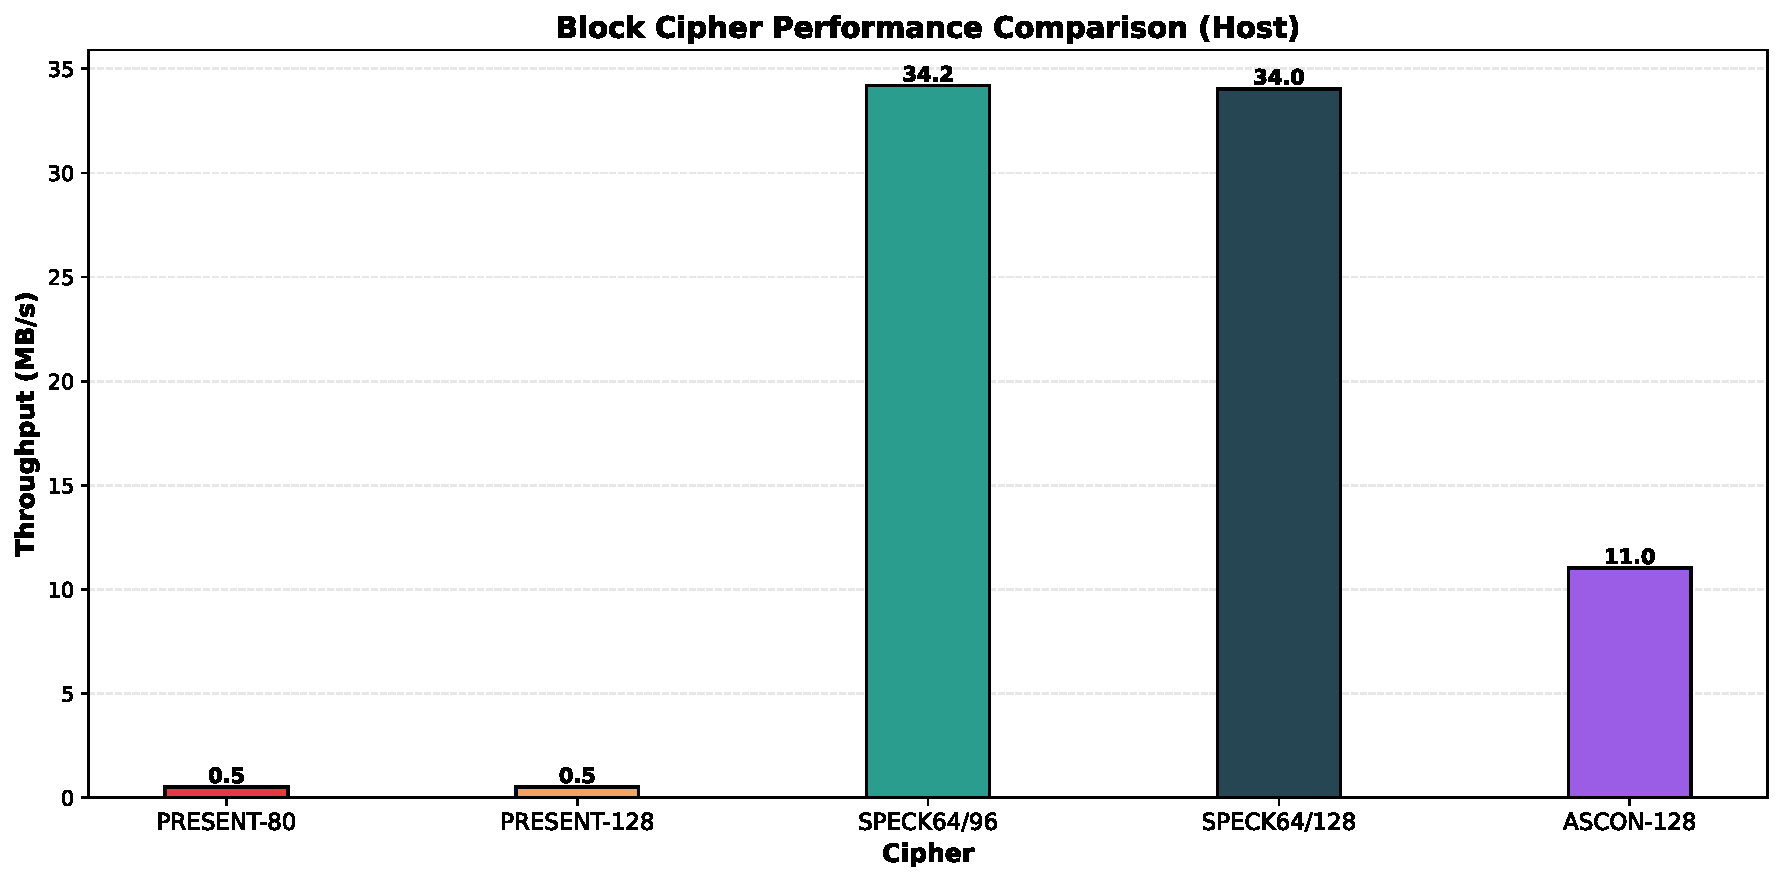
\includegraphics[width=0.9\textwidth]{block_cipher_comparison.pdf}
    \caption{Performance Comparison: PRESENT, SPECK, ASCON}
    \label{fig:block-cipher-comparison}
\end{figure}

\subsection{Mode Comparison}

\begin{figure}[H]
    \centering
    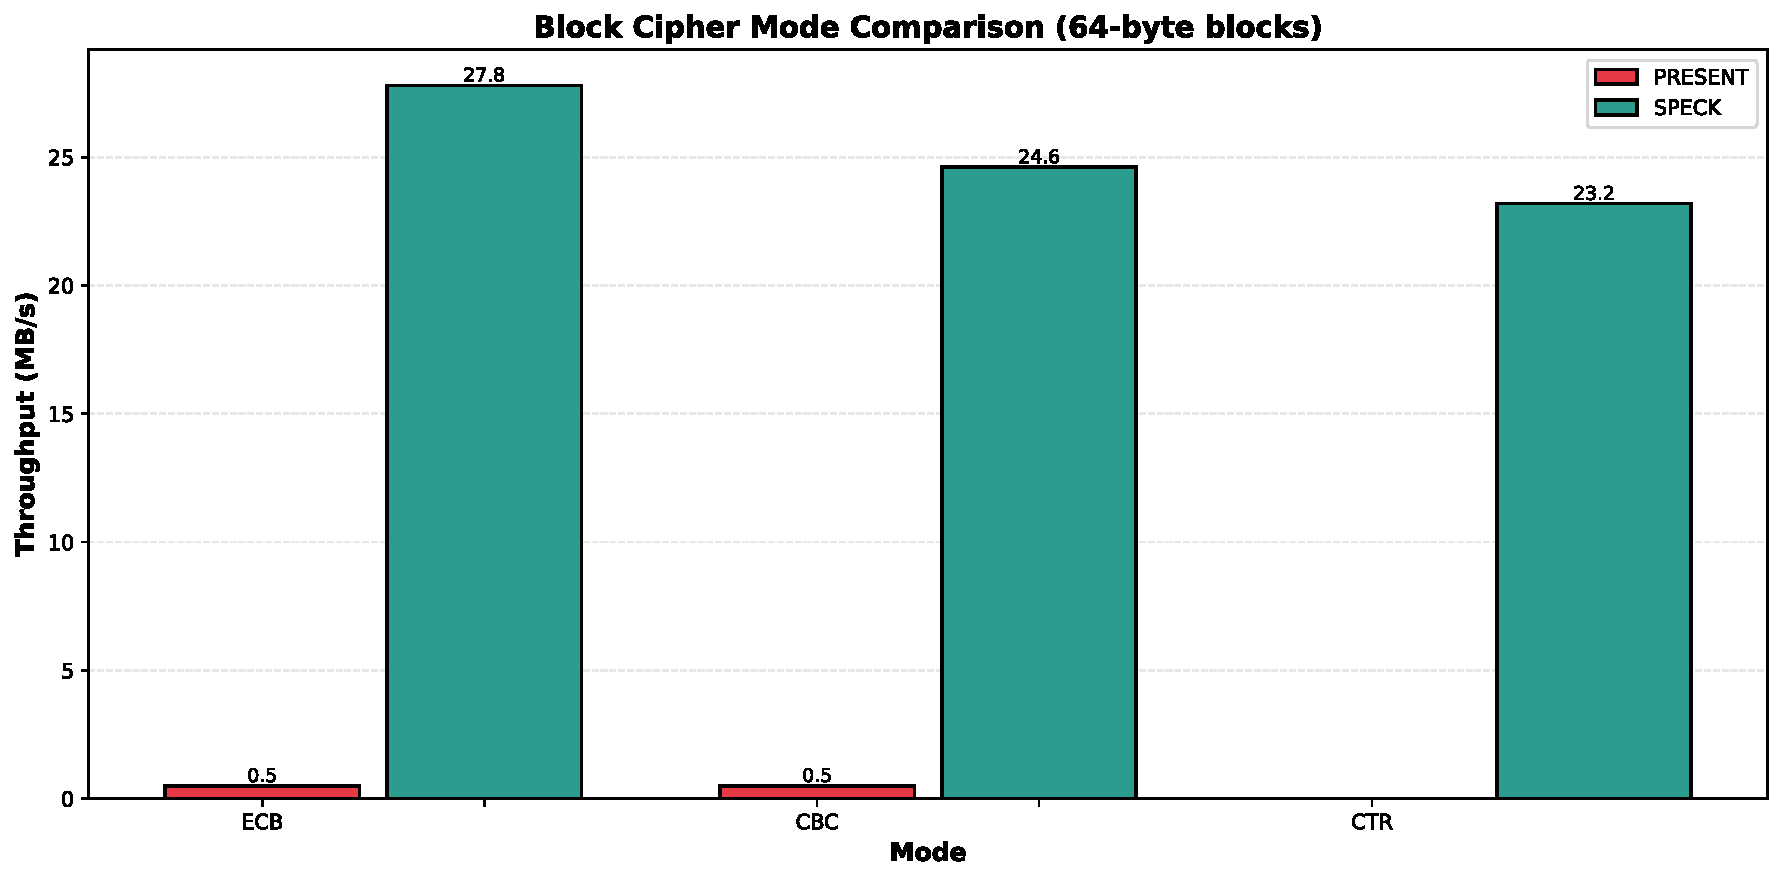
\includegraphics[width=0.9\textwidth]{mode_comparison.pdf}
    \caption{ECB vs CBC vs CTR Mode Performance}
    \label{fig:mode-comparison}
\end{figure}

\subsection{ASCON Phase Breakdown}

\begin{figure}[H]
    \centering
    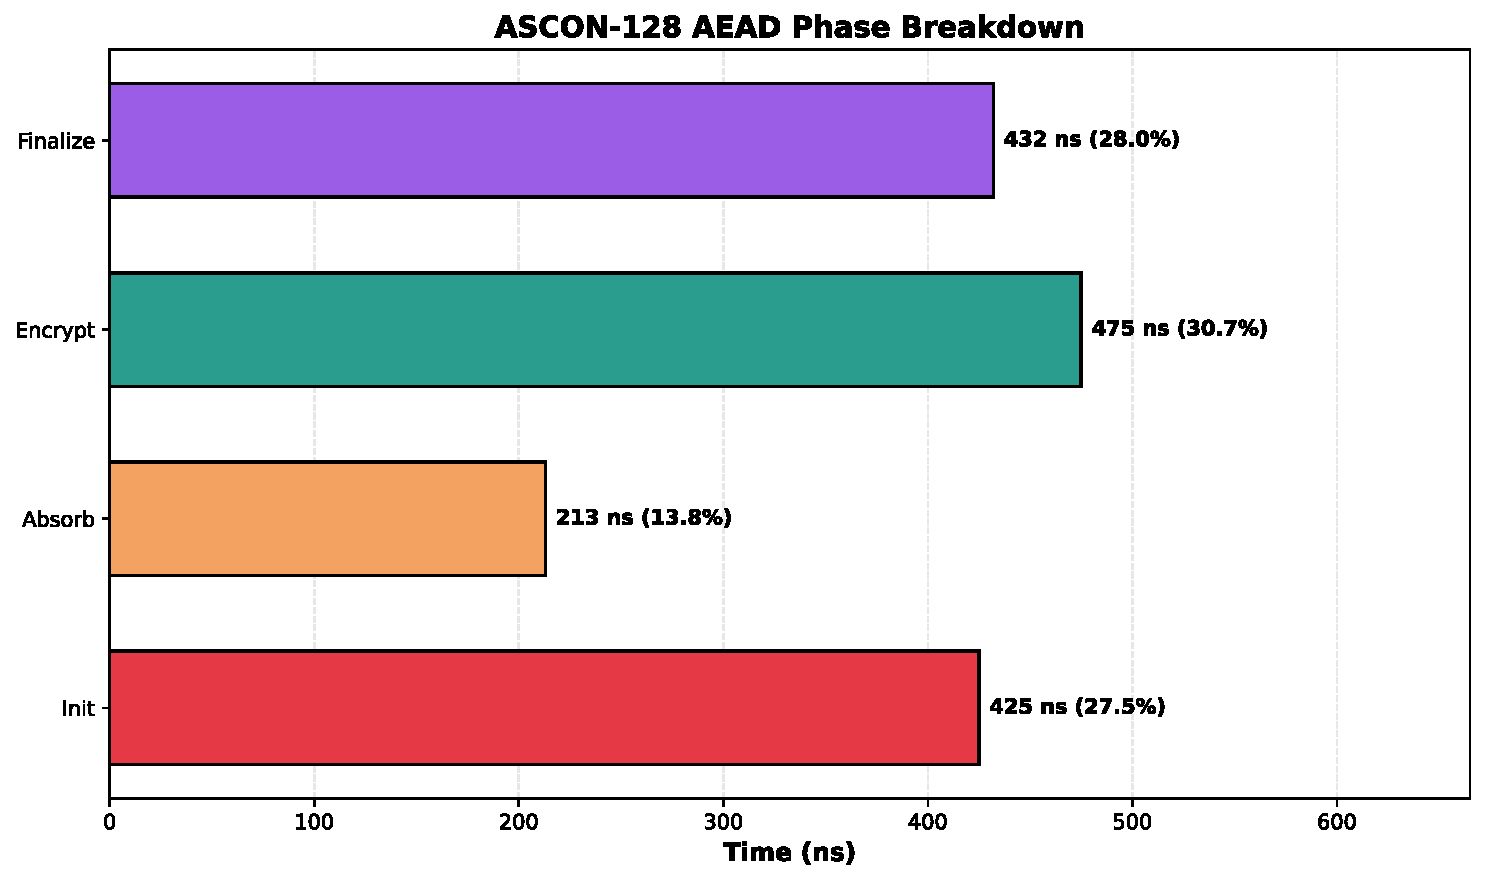
\includegraphics[width=0.9\textwidth]{ascon_breakdown.pdf}
    \caption{ASCON AEAD Phase Performance}
    \label{fig:ascon-breakdown}
\end{figure}

\subsection{Scaling Analysis}

\begin{figure}[H]
    \centering
    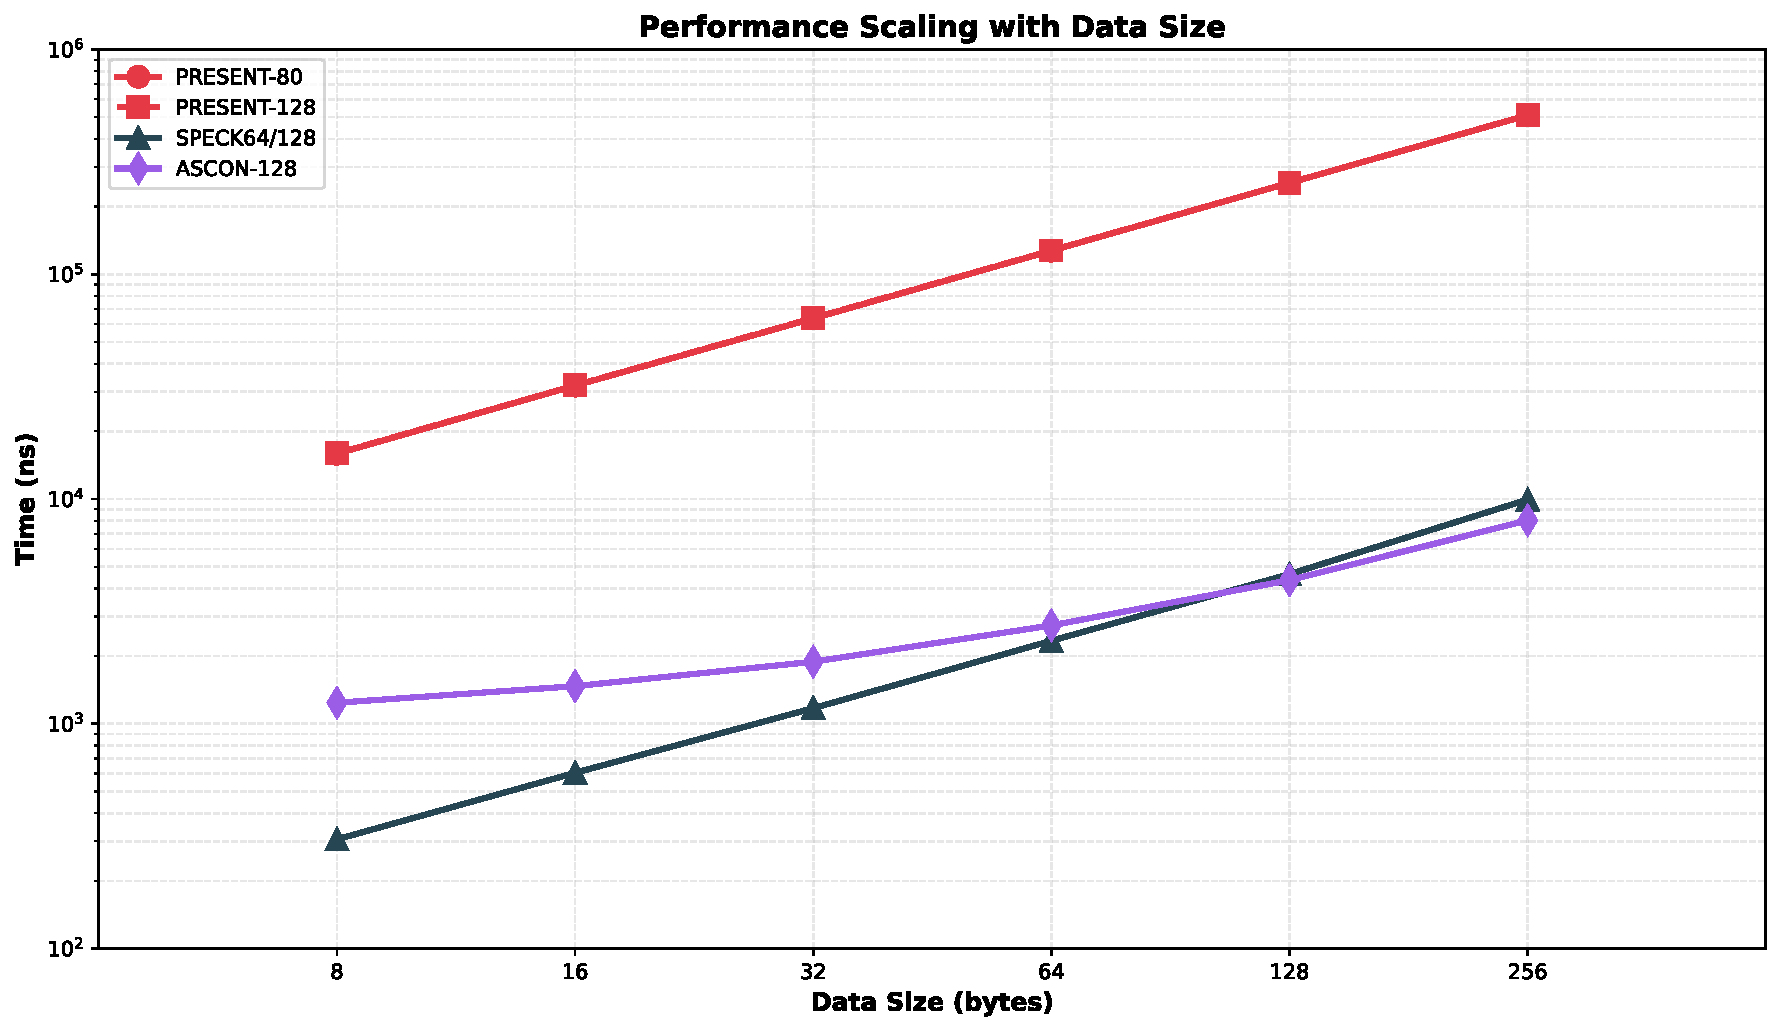
\includegraphics[width=0.9\textwidth]{scaling_analysis.pdf}
    \caption{Performance vs Block Size (8-256 bytes)}
    \label{fig:scaling-analysis}
\end{figure}

\section{Analysis}

\subsection{Performance Observations}

\begin{itemize}
    \item \textbf{SPECK} is the fastest: 23.67 Mbps on Pico, approximately 70x faster than PRESENT
    \item \textbf{ASCON} provides good balance with built-in authentication (7.56 Mbps on Pico)
    \item \textbf{PRESENT} is the slowest on software but designed for hardware efficiency
    \item CTR mode offers best performance among encryption modes for SPECK
    \item ASCON's initialization overhead is amortized over larger message sizes
\end{itemize}

\subsection{Memory Analysis}

Based on code size analysis:
\begin{itemize}
    \item \textbf{SPECK} has the smallest ROM footprint due to ARX-only operations (no lookup tables)
    \item \textbf{PRESENT} requires additional storage for S-box tables but remains compact
    \item \textbf{ASCON} has the largest code size due to 320-bit state and complex permutations
\end{itemize}

These results demonstrate that SPECK is optimal for performance-critical applications, while PRESENT suits hardware-constrained environments, and ASCON provides the best security-to-performance ratio for authenticated encryption needs.

\chapter{Conclusion and Future Work}

\section{Conclusion}

This study investigates lightweight cryptographic algorithms tailored for resource-constrained embedded platforms. A literature review highlights the emergence of lightweight approaches driven by IoT deployment challenges.

Three representative algorithms—PRESENT, SPECK, and ASCON—were selected to evaluate performance, memory efficiency, and theoretical security strength. The proposed methodology enables a structured comparison using Rust-based implementations on the Raspberry Pi Pico.

Results show that SPECK provides superior performance, PRESENT offers minimal memory footprint, and ASCON delivers strong modern security with functional completeness. Algorithm selection in embedded systems must therefore align with specific application needs and deployment constraints.

This report establishes a foundation for empirical benchmarking and provides methodological guidelines for further work.

\section{Future Work}

Future research can extend this study in the following directions:

\subsection{Short-Term}

\begin{itemize}
    \item \textbf{NIST KAT Tests}: Integrate official Known Answer Test vectors
    \begin{itemize}
        \item PRESENT: ISO/IEC 29192-2 test vectors
        \item SPECK: NSA-designed test vectors
        \item ASCON: NIST LWC standardization test vectors
    \end{itemize}
    \item \textbf{Code Size Analysis}: Static analysis for .text/.data/.bss sections using cargo size
    \item \textbf{Statistical Rigor}: Report median/min/max across multiple benchmark runs instead of single run
\end{itemize}

\subsection{Medium-Term}

\begin{itemize}
    \item \textbf{FELICS Comparison}: Compare against established lightweight crypto benchmarks (felics.eu)
    \item \textbf{SUPERCOP-Style Timing}: Implement cycle-accurate benchmarking methodology
    \item \textbf{Side-Channel Discussion}: Analyze timing attack resistance for ARX ciphers (SPECK)
\end{itemize}

These directions will deepen the understanding of lightweight cryptographic design and facilitate secure IoT-system development.

\end{document}
